\documentclass[12pt,a4paper,openany]{book}

%Uporabljeni paketi
\usepackage[utf8]{inputenc}
\usepackage{cmap}
\usepackage{type1ec}
\usepackage[T1]{fontenc}
\usepackage{fancyhdr}
\usepackage{graphicx,epsfig}
\usepackage[english]{babel}
\usepackage{cite}
\usepackage{caption} % improve caption spacing (among other things)
\usepackage{subcaption}
\usepackage[pdftex,colorlinks,citecolor=black,filecolor=black,linkcolor=black,urlcolor=black,pagebackref]{hyperref}
\usepackage{tikz}
\bibliographystyle{ieeetr}

%Velikost strani - dvostransko
\oddsidemargin 1.4cm
\evensidemargin 0.35cm
\textwidth 14cm
\topmargin 0.26cm
\headheight 0.6cm
\headsep 1.5cm
\textheight 20cm

%Nastavitev glave in repa strani
\pagestyle{fancy}
\fancyhead{}
\renewcommand{\chaptermark}[1]{\markboth{\textsf{Chapter \thechapter:\ #1}}{}}
\renewcommand{\sectionmark}[1]{\markright{\textsf{\thesection\  #1}}{}}
\fancyhead[RE]{\leftmark}
\fancyhead[LO]{\rightmark}
\fancyhead[LE,RO]{\thepage}
\fancyfoot{}
\renewcommand{\headrulewidth}{0.0pt}
\renewcommand{\footrulewidth}{0.0pt}

\newcommand{\gnuplot}{\textbf{gnuplot}}
\newcommand{\pgfname}{\textsc{pgf}}
\newcommand{\tikzname}{Ti\emph{k}Z}

%%%%%%%%%%%%%%%%%%%%%%%%%%%%%%%%%%%%%%%%%%%%%%%%%%%%%%%%%%%%%%%%
%% ccBeamer 0.1, 2007-07-02                                   %%
%% Written by Sebastian Pipping <webmaster@hartwork.org>      %%
%% ---------------------------------------------------------- %%
%% Licensed under Creative Commons Attribution-ShareAlike 3.0 %%
%% http://creativecommons.org/licenses/by-sa/3.0/             %%
%%%%%%%%%%%%%%%%%%%%%%%%%%%%%%%%%%%%%%%%%%%%%%%%%%%%%%%%%%%%%%%%


%% Images
\newcommand{\CcImageBy}[1]{%
	\includegraphics[scale=#1]{creative_commons/cc_by_30.pdf}%
}
\newcommand{\CcImageCc}[1]{%
	\includegraphics[scale=#1]{creative_commons/cc_cc_30.pdf}%
}
\newcommand{\CcImageDevNations}[1]{%
	\includegraphics[scale=#1]{creative_commons/cc_dev_nations_30.pdf}%
}
\newcommand{\CcImageNc}[1]{%
	\includegraphics[scale=#1]{creative_commons/cc_nc_30.pdf}%
}
\newcommand{\CcImageNd}[1]{%
	\includegraphics[scale=#1]{creative_commons/cc_nd_30.pdf}%
}
\newcommand{\CcImagePd}[1]{%
	\includegraphics[scale=#1]{creative_commons/cc_pd_30.pdf}%
}
\newcommand{\CcImageSa}[1]{%
	\includegraphics[scale=#1]{creative_commons/cc_sa_30.pdf}%
}
\newcommand{\CcImageSampling}[1]{%
	\includegraphics[scale=#1]{creative_commons/cc_sampling_30.pdf}%
}
\newcommand{\CcImageSamplingPlus}[1]{%
	\includegraphics[scale=#1]{creative_commons/cc_sampling_plus_30.pdf}%
}


%% Groups
\newcommand{\CcGroupBy}[1]{% zoom
	\CcImageBy{#1}%
}
\newcommand{\CcGroupByNc}[2]{% zoom, gap
	\CcImageBy{#1}\hspace*{#2}\CcImageNc{#1}%
}
\newcommand{\CcGroupByNcNd}[2]{% zoom, gap
	\CcImageBy{#1}\hspace*{#2}\CcImageNc{#1}\hspace*{#2}\CcImageNd{#1}%
}
\newcommand{\CcGroupByNcSa}[2]{% zoom, gap
	\CcImageBy{#1}\hspace*{#2}\CcImageNc{#1}\hspace*{#2}\CcImageSa{#1}%
}
\newcommand{\CcGroupByNd}[2]{% zoom, gap
	\CcImageBy{#1}\hspace*{#2}\CcImageNd{#1}%
}
\newcommand{\CcGroupBySa}[2]{% zoom, gap
	\CcImageBy{#1}\hspace*{#2}\CcImageSa{#1}%
}
\newcommand{\CcGroupDevNations}[1]{% zoom
	\CcImageDevNations{#1}%
}
\newcommand{\CcGroupNcSampling}[2]{% zoom, gap
	\CcImageNc{#1}\hspace*{#2}\CcImageSampling{#1}%
}
\newcommand{\CcGroupPd}[1]{% zoom
	\CcImagePd{#1}%
}
\newcommand{\CcGroupSampling}[1]{% zoom
	\CcImageSampling{#1}%
}
\newcommand{\CcGroupSamplingPlus}[1]{% zoom
	\CcImageSamplingPlus{#1}%
}


%********************************************

\begin{document}

% stran 1 med uvodnimi listi
\thispagestyle{empty} 

\begin{center}
{\large 
IMPERIAL COLLEGE LONDON \\
DEPARTMENT OF COMPUTING\\
}

\vspace{3cm}
{\LARGE Pedro Kostelec}\\
CID: 00655960\\

\vspace{2cm}
\textsc{\textbf{\LARGE 
Cell Tracking methods 
}}

\vspace{2cm}
{ LITERATURE SURVEY }

\vspace{2cm} 
{\Large Supervisor: Ben Glocker}

\vfill
{\Large London, May 2014}
\end{center}


%********************************************

% stran 2 med uvodnimi listi
\thispagestyle{empty}

\newpage


%********************************************


\renewcommand\thepage{} 
\tableofcontents 
\renewcommand\thepage{\arabic{page}}

\thispagestyle{empty}

\chapter{Introduction}
This literature survey describes the background research that has been completed in preparation for the work on the project entitled ``Automatic Cell Tracking and Categorisation for Microscopic Image Analysis''.

Quantitative analysis of cell populations using time-lapse microscopy is important for understanding cell behaviour. This analysis requires tracking a large number of cells in often low quality image sequences of varying contrast. Often then most effective way to do this is to manually annotate each cell in every frame of the sequence. However, this is slow and tedious, thus limiting the amount of data that we are able to analyse. Several computer vision algorithms have been developed to reduce the amount of manual work required for the analysis of large time-lapse sequences. Ideally, we would like to develop an algorithm that is able to track any type of cells in image sequences, regardless of the imaging technique used to capture them. However, the current state-of-the-art in computer vision is unable to perform this task accurately and automatically. For this reason, several algorithms have been developed to handle specific cases, relying on heuristics to improve their performance.

The main emphasis of this project is to track leukocytes in low quality image sequences acquired with fluorescent reporter technology and light microscopy. Additionally, the behaviour of these cells with be quantified to allow for further studies of leukocytes.

This is a joint project with Dr. Leo Carlin from the Leukocyte Biology Section at the National Heart and Lung Institute (NHLI) and is supervised by Dr. Ben Glocker.

The remaining of the report is divided into two chapters. Chapter \ref{chap:methodoverview} summarizes the essential material related to cell detection and tracking. In the Chapter \ref{chap:workplan} we present an informative work plan that will guide the development of the software. 



\chapter{Cell tracking methods}
\label{chap:methodoverview}

This chapter is an overview of the background research that has been completed in preparation for the work on the project. The chapter is divided into four sections. Section \ref{sec:detection} describes methods to perform cell detection on cell images. Section \ref{sec:tracking} presents methods used to track cells in a sequence of images. Finally, in Section \ref{sec:conclusionmethods} we describe which methods seem most promising and discuss reasons why the use of automated cell tracking methods is not as widespread as we would be led to believe, given the wide range of research that has been done on the subject.


\section{Cell detection}
\label{sec:detection}

Cell detection consists in identifying individual cells in microscopy images. Due to the different imaging techniques and the types of cells we may wish to detect, several algorithms have been developed each to handle a specific case. This section is an overview of these techniques.

\subsection{Cell segmentation using the Watershed technique}

A basic cell detection method relies in binarizing an image to separate the background from the cells, followed by a segmentation step to extract the cells. The approach presented in \cite{chen99} is as follows:

\begin{enumerate}
  \item Apply a spatial adaptive filter to the image to minimize the effect of noise.
  \item Locate the pixels with minimum intensities in a small sliding window.
  \item For each minimum point we proceed to the progressive flooding of its neighbouring points
  \item Post-processing step to discard false regions.
\end{enumerate}

A more modern, yet similar, approach would perform binarization with Otsu's threshold selection method \cite{otsu79}, followed by some morphological operations \cite{serra83} to fill holes and eliminate patches that are too small to correspond to cells, and finally use the Watershed algorithm \cite{beucher79} to segment the binary image into individual cells. The disadvantage of this method is that the number of pixels belonging to either cells or background should be approximately the same, and that the signal-to-noise ratio should be low.

Chen et al \cite{chen06} have used an improved Watershed algorithm \cite{vincent93} to separate cell nuclei after using Otsu's thresholding method to segment nuclei from the background. Additionally they developed a nuclei-fragment merging method based on he shapes and sizes of the nuclei to deal with the problem of over-segmentation caused by the Watershed algorithm.


\subsection{Cell segmentation using level sets}

Another interesting technique to segment cells is a contour evolution method that makes use of the general appearance of cells to segment them using level sets. Mukherjee \cite{mukherjee04} makes the observation that leukocyte shapes are nearly circular cells and that at least for a significant part of the border of the cell, the intensity profile is different from the cell cytoplasm and from the background. Using this observation, identification of a leukocyte is formulated as a minimization of an energy function incorporating image gradient and intensity homogeneity within the closed contour encompassing the cell. The benefit of this method is that it can be adjusted to perform well in images with significant clutter and poor contrast by increasing the importance of the homogeneity, or for images with good contrast, where the gradient magnitude term is given more importance. The disadvantage of this method is that cells cannot overlap. The energy function can be minimized with the gradient descent method.

To reduce the solution space for the energy function only the boundaries of connected components within the image-levels sets are evaluated with the energy function. Only the connected components satisfying the size and shape constraints of the cells are extracted. The remaining components are eliminated using area morphology operations. This level-set analysis provides a more efficient solution that is linear in the number of intensity levels in the image in contrast to the much higher complexity of a curve evolution method.

The level set method is contour evolution approach which has good results in segmentation. Tang et al \cite{Tang??} have successfully level-sets combined with local grey thresholding \cite{xu10} for neuron stem cells images which have been obtained by confocal microscopy.

\subsection{Cell detection by model learning}

The previous methods perform efficiently in cells with sufficiently good contrast. In images where the cell borders are unclear, images are of varying intensity, cell density is high, or cells can be of different shapes, these methods would not perform as well. In such cases machine learning methods can perform better by learning a model of a cell based on a large number of annotated examples.

Arteta et al \cite{arteta12}\cite{arteta13},  propose an algorithm that uses a highly-efficient MSER region detector \cite{matas02} to find a broad number of candidate regions. These regions are then scored depending on the similarity to the cell type of interest by a machine learning algorithm. 

The authors organized the extremal regions obtained from the MSER detector into trees, so that each tree corresponds to a set of overlapping extremal regions. The non-overlapping regions which achieve high scores can then be selected using dynamic programming of the trees. Two learning strategies are tested: a binary classifier using Support Vector Machines (SVM) and structured learning (structured SVM \cite{joachims09}) which is able to take into account the non-overlap constraint, and achieves better performance.

The feature vector for each regions is composed of several concatenated histograms: a histogram of intensities within the region, two histograms of differences in intensities between the region border and a dilation of it for two different dilation radii, a shape descriptor and the area of the region. The downside of this approach is that extracting the feature vector from the image is slow, especially because it needs to be extracted for each image in the sequence.

The advantage of this approach is the tolerance to changes in image intensities, cell densities and sizes. The major downside is the non-overlap constraint. Fortunately the authors have also developed an algorithm to detect partially overlapping cells \cite{arteta13}. 

The idea is to learn to detect overlapping cells, and the number of cells in the region. The algorithm starts by generating a set of nested regions. Each region is then scored using a set of classifiers that evaluate the similarity of the region to each of the possible classes, where each class corresponds to the number of cells that the region contains. An inference procedure then selects the non-overlapping subset of regions, and assigns each a class label indicating the number of cells that the model believes lie in the region. 

\subsection{Cell detection by image restoration}

Another approach is to use an image restoration technique followed by thresholding \cite{bise11} \cite{huh13}. Bise et al \cite{bise11} apply this technique on phase-contrast microscopy images . The technique utilizes the optophysical principle of image formation by phase-contrast microscope to transform the image into an artefact free image by minimizing a regularized quadratic cost function. After this, a simple image thresholding technique can be used for segmentation.

\section{Cell tracking}
\label{sec:tracking}

After detecting each cell in each image of the sequence we need to determine which cells in an image correspond to which in the next image. This way we can generate a track of the cell across the sequence. This is the problem of tracking. There are three main approaches to tracking:

\begin{description}
	\item [Tracking by model evolution] Active contours or level sets are used to detect a cell in the first frame of the sequence, and the initial points are then propagated to the next frame. This method can be computationally expensive because of the need to evolve the cell models for each frame.
	\item [Tracking by data association] Cells in consecutive frames are associated according to a similarity measure, which compares features such as the cell intensity of relative spatial location. This method requires very accurate segmentation to perform well.
	\item [Tracking with a dynamics filter] This method uses a dynamics filter (e.g. Kalman or Particle filter) to predict the spatial location of the cell in the next frame.
\end{description}

The remaining of this chapter describes how this methods have been implemented in different papers.

\subsection{Tracking by model evolution}

Model evolution tracking methods handle cell deformation well, but can often get stuck in local minima. It is possible to improve the tracking accuracy at the expense of computation time.

Mukherjee \cite{mukherjee04} models the problem of cell tracking as maximizing a similarity measure between level sets in consecutive frames. The method minimizes the energy associated with leukocyte boundary detection and then match the boundary with that of the previous frame. To maintain spatial coherence, the authors assume that the displacement of cells between frames is marginal. Such an automatic tracker is able to handle slight rotations or deformations of the leukocytes well.

\subsection{Tracking by data association}

When tracking by data association, cells in consecutive frames are associated according to a similarity measure, which compares features such as the cell intensity or relative spatial location. This method is very efficient, but only effective when cells are accurately detected. It is possible to improve the association by analysing several frames in a sequence.

Chen et al \cite{chen06} perform the matching process based on the distances between the cells. An association matrix is built based on the Euclidean distance between cell nuclei and their sizes. A match is found if the distance is below a threshold. Four possible outcomes are possible in this matching process:

\begin{enumerate}
	\item A successful one-to-one match is identified.
	\item A nucleus moves out of the field of view, which can only happen in the borders.
	\item Nucleus separation.
	\item Several nuclei in one frame match a single nucleus in the following frame. This can be the result of under-segmentation.
\end{enumerate}

To overcome the problem of false matches, the following procedure is applied. For the fourth case, the true candidates are selected by finding the candidates whose aggregated size matches the `one' nucleus most closely. A similar procedure is used for one-to-many correspondences.

A strategy is developed to resolve the issue of ambiguous correspondence when nuclei are touching or partially overlapping. In this case information (nuclei size and their relative location -- up, down, left, right --) about these nuclei is stored. When they separate, the algorithm can resolve the ambiguities by comparing their current status with the previously stored information.

Over-segmentation is resolved by merging fragments if the sum of sizes of the close fragments corresponds to the size of a nucleus in the previous frame.

Cells that undergo division or occlude other cells make the problem of tracking harder. Baker et al \cite{baker13} used a contour-based segmentation method. Cells with a common contour are tagged as siblings and undergo additional tests to determine if they are part of division or occlusion events based on whether both cells existed previously or not. Occlusions are further examined with a positional cost function and mislabelled cells are corrected.

Cell division detection is crucial for developing a high accuracy tracking algorithm in cell populations where mitosis is frequent, as is demonstrated in \cite{huh13}. Based on the segmented blobs in the previous frame frame-by-frame data association is performed in the current frame. The authors categorized five hypothesis about cell behaviour: migration, exit, entrance, clustering and mitosis. The hypothesis regarding mitosis detection often produces too many false positives, and sometimes may not detect mitosis even if it should. To mitigate this effect, a cell mitosis detection algorithm is run independently on the image sequence. The mitosis hypothesis is only evaluated for the cells that have been discovered by this algorithm. After all hypothesis are obtained, a best combination is selected by formulating and solving an integer programming problem. If, after the best association is found, there are remaining cells, these are considered again in the following frames. The association is attempted for the following 10 cells before the track is marked as terminated. A similar method is used to generate new tracks for newly detected cells. Each such cell generates a temporary track, which is confirmed as real track if the track is associated in the majority of the following 10 frames.

The similarity function used to perform data association between images is of crucial importance. House et al \cite{house09} propose a novel cost function that encodes the response of cells to conditions of their environment. The tracking problem is formulated as a standard Bayesian filtering problem. The model allows the state of the cells in the image to evolve in time. To solve the complete assignment two algorithm are evaluated: an iterative probabilistic data association algorithm, which produces an optimal solution, and a two-phase batch algorithm, which produces a suboptimal solution. The performance of both algorithms is dependent on the cost function used. The authors propose and evaluate three different cost functions. The two-phase batch algorithm has difficulties when cells occlude each other, or die or divide in close proximity to another. It performs very well in low-density population with few events occurring. The optimal algorithm, which performs much better in these harder scenarios, has had most difficulties in matching daughter cells to their parent cell.


\subsection{Tracking with a dynamics filter}

Dynamics filters are a powerful addition to tracking systems because they predict the motion of a cell, and reduce the search space in which we look for matches. These algorithms not only perform frame-by-frame tracking, but also take temporal information into account, resulting in more accurate tracking performance.

Xu et al \cite{xu12} developed an ant stochastic searching behaviour based tracking system to track multiple cells in fluorescent image sequences. The system is similar to particle filters, but the motion behaviour is modelled to be similar to how ant behave when searching for food. When ants move around, they deposit small quantities of chemical pheromone. Once they find food, they retrace the steps deposing larger amounts of pheromone. Other ants can the use this guide to find food faster, but are allowed to deviate from the path and pursue their own paths. The author propose a system where the food is not static, so that it can be used for cell tracking. The algorithm is as follows. The predicted state of each an is computed based on a dynamic model. Then the importance weights for the predicted states are normalized. An ants moves first in its predicted state. Afterwards, its moving direction can be influenced by the states of other ants. When the ants finish their path selections, the pheromone update process takes place. In this algorithm the updated pheromone refers to the moving ability of an ant. Ants with larger weights are located closer to the food, and move slower. Ants with lower weights are further away from food and move more aggressively.

Compared to particle filters, this algorithm is more computationally expensive, but achieve better accuracy. The algorithm is able to deal with cells entering or leaving the scene, and occlusion.

Kalman filters are another popular method for state prediction. Tang et al \cite{tang} use a Kalman filter to guide the tracking of active cells. Active cells are those that move a distance larger than L (supposedly their radius) between frames. Inactive cells are tracked by observing the overlap region. The state vector is composed of the cell two dimensional position and the corresponding velocities. The system external input vector is composed of the acceleration in two dimensions. To initialize the Kalman filter, the cells are first tracked in the first three frames by means of a similarity function evaluated in neighbouring locations in successive frames. From the third frame onward, the Kalman filter is used to predict the cell's location and reduce the search space.

Cell do not always exhibit just one type of motion and a single Kalman filter cannot take this into account. Li et al \cite{li07} propose an automated tracking system which runs several Kalman filters in parallel, each corresponding to a different modality. Their system is composed of five modules: cell detector, cell tracker, dynamics filter, track compiler and track linker.

The cell detector separates the background from cell pixels. The cell tracker propagates the cell labelling to the next frame in the sequence. The track compiler compares the results of the cell tracker, cell detector and dynamics filter to create a new track for new or daughter cells, update or terminate existing tracks. The track linker connects two or more track segments if they belong to the same cell. 

Several assumption are made regarding the appearance and motion of the cells. First they are approximately elliptic in shape. Second, their position and intensity change are governed by independent processes. Third, the dynamic processes governing each cell are independend. Suppose that the cellular motion consists of a finite number of modes. The interacting multiple models (IMM) filter operates several Kalman filters in parallel, each modelling a different mode of motion. The transition between models is determined by a finite state Markov chain. The author use three models of cell dynamics: random walk, first-order and second-order linear extrapolation which correspond to Brownian motion, migration with constant speed and migration with constant acceleration. To initialize the IMM filter the system tracks the cells each cell in the first three frames in which they appear. The parameters of the model are estimated offline using the Expectation-Maximization algorithm.

This model is robust to long-term occlusion and cell detection error.

\subsection{Cell tracking as a network flow problem}

Massoudi et al \cite{massoudi12} propose a tracking method that does not rely on perfect segmentation and can deal with uncertainties by exploiting temporal information and aggregating the results of many frames. The system only requires probabilities or potentials that represent cell positions. Tracking is modelled as a network flow problem and is formulated as a linear program based on the occupanty likelihood of the edges of the network. The benefit of this approach is that it aggregates the results of all frame and makes a global decision rather than propagating the results of each frame to the next, which makes it less dependent on the cell detection module. The system can detect false positives or false negatives and correct itself. The method handles division events, cells entering or exiting the screen at the boundaries.

\section{Conclusion}
\label{sec:conclusionmethods}
This chapter presented an overview of methods used for cell detection and tracking. In the future, specific methods will be selected and analysed based on the quality of image sequences that we will be analysing. The small sample of images made available in the past week by Dr Leo Carlin show low contrast cells and rapidly changing morphology. The images were low quality so that basic computer vision techniques will probably not suffice for efficient cell segmentation and tracking. First some image restoration preprocessing steps will need to be performed to reduce the artefacts caused by the imaging method. It seems that a machine learning approach, similar to \cite{arteta13} will be most effective to detect the cell position. According to Dr. Leo Carlin, few or no mitosis events will be present in the image sequences that we will study, so a section on mitosis detection has been left out of this literature survey. Because of the low quality images a data association approach will probably not be very accurate for tracking. A dynamic filter approach will most likely be used.

There are several reasons why automatic cell tracking systems are not as popular as we would expect. The main reason is probably that the level of accuracy falls short of manual annotation. Furthermore, these systems are often not robust to changes in cell type, cell culture condition and microscopy image quality. The goal of this research is to develop a system that can track leukocytes in low quality images with an accuracy that is similar to that of a human. 


\chapter{Work plan}
\label{chap:workplan}

In order to complete the project in due time, a work plan is outlined to guide the development of the software.

The first phase of the project was background literature research and an overview of the learned methods and techniques is outlined in the previous chapter. Additionally, I have also performed background research on cell mitosis. These notes are not included in this background survey, because according to Dr. Leo Carlin the image sequences we will study have few or no mitosis events.

\section{Architecture}

Similar to the work by Li et al \cite{li07}, a modularized approach is going to facilitate development and testability of the software. This approach has the benefit that any of the modules could be swapped without affecting the other parts of the system. Li et al have used the following modules: Cell Detector, Cell Tracker, Dynamics Filter, Track Compiler and Track Linker. These modules will be used as a guideline when developing our own version of the tracker for leukocytes. However, not everything will be the same. For example, their approach connects the Track Compiler to the Cell Detector modules, because the Track Compiler is able to provide the Cell Detector updated histograms that the Cell Detector uses for detection using a Bayesian classifier. This relationship is only necessary if the learning is done on-line, that is if the Cell Detector module is able to use these updated histograms to better detect new cells in the following images.

For the Cell Detector module, an off-line learning approach will probably be tested, similar to the one in \cite{arteta12}\cite{arteta13}. However the details will only be defined once sufficient sample image sequences are analysed.

An additional module will be developed to quantify the behaviour of the cells over time. Cell displacement, the proportion of time they more in close proximity to other cells, the changes of cell velocity over time, ... are example of measurements that it will be responsible for.

The program will be developed in MATLAB and will include an executable GUI that will permit the user to use the application without the entire MATLAB package.

\section{Image sequences}

Up to date, only one sample of an image sequence was made available. The data is provided by Dr. Leo Carlin from the Leukocyte Biology Section at the National Heart and Lung Institute (NHLI). He has promised to provide more data as soon as it is obtained.

TODO add border in between
\begin{figure}
\centering
\begin{subfigure}{.5\textwidth}
  \centering
  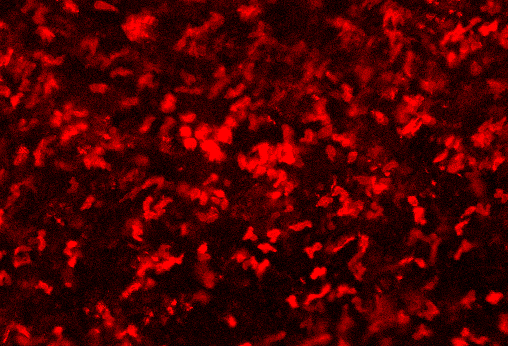
\includegraphics[width=\textwidth]{frame1.png}
  \caption{}
\end{subfigure}%
\begin{subfigure}{.5\textwidth}
  \centering
  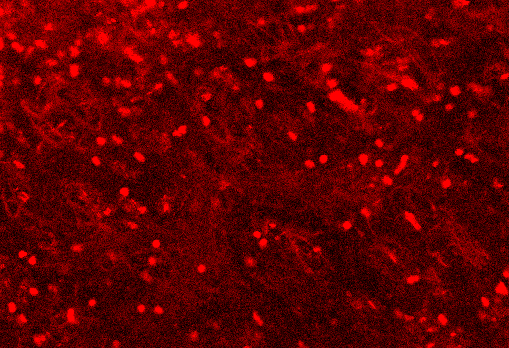
\includegraphics[width=\textwidth]{frame2.png}
  \caption{}
\end{subfigure}
\caption{Two example frames of cell images that the tracker will need to successfully process and track the individual cells. The colour of the images has been enhanced for this display.}
\label{fig:sampleframes}
\end{figure}

Figure \ref{fig:sampleframes} displays two sample frames from the provided image sequence. The images are low quality, and the cell borders have low contrast. Obtaining more sample data is crucial to be able to shortlist which algorithms are appropriate for accurate cell detection and tracking.

\section{Development schedule}

The following is a rough outline of a work plan. This is a preliminary plan, which will be adjusted as work progresses.

\begin{enumerate}
  \item [May] Focus will be on developing cell detection algorithms (the Cell Detection module). For this purpose a basic annotation program may also be written, which should ease annotating image sequences by clicking on cells.
  \item [June] A basic tracking system that will track cells over time (the Cell Tracker module). Additionally, a module to compute interesting statistics of cell tracks will be developed. If there will be excess time, a Dynamics filter module will be developed.
  \item[July] Focus will be on developing other modules as necessary, for example a Track Compiler and Track Linker. Also, the Cell Detection and Tracking modules will be improved if needed.
  \item [August] Writing a GUI for the software, testing and writing the final report.
\end{enumerate}

%********************************************

\newpage


\addcontentsline{toc}{chapter}{Bibliography}
\label{page_bibliography}
\bibliography{survey} 



\end{document}




